% $Id: INF_Poster_example.tex 7714 2011-08-31 17:34:46Z tkren $
%
% TU Wien - Faculty of Informatics
% poster template
%
% This template is using the beamer document class and beamerposter package, see
% <http://www.ctan.org/tex-archive/macros/latex/contrib/beamer/>
% <http://www.ctan.org/tex-archive/macros/latex/contrib/beamerposter/>
% <http://www-i6.informatik.rwth-aachen.de/~dreuw/latexbeamerposter.php>
%
% For questions and comments send an email to
% Thomas Krennwallner <tkren@kr.tuwien.ac.at>
%

\documentclass[final,hyperref={pdfpagelabels=true}]{beamer}

\usepackage{TUINFPST}   			% Poster template
\usepackage{algorithm}  			% For algorithms
\usepackage[noend]{algpseudocode} 	% Allows pseudo-code like syntax in algorithms
\usepackage{caption}				% Better caption handling
\usepackage{ragged2e}				% Alignments
\usepackage[export]{adjustbox}		%For aligning images right and left
\usepackage{multicol}				%Multicolumn environment (for bibliography)

%\title[Computational Intelligence]{Interactive Computer Generated Architecture}
% if you have a long title looking squeezed on the poster, just force
% some distance:
\title[\protect\parbox{.65\textwidth}{Software Engineering \& Internet Computing}]{%
  Context Enrichment of \\[0.2\baselineskip]%
  Crowdsourcing Tasks for \\[0.2\baselineskip]%
  Ontology Validation
}
\author[stefan.gamerith@gmx.com]{Stefan Gamerith}
\institute[]{%
  Technische Universit{\"a}t Wien\\[0.25\baselineskip]
  Institut f{\"u}r Softwaretechnik und Interaktive Systeme\\[0.25\baselineskip]
  Arbeitsbereich: Information \& Software Engineering Group\\[0.25\baselineskip]
  Betreuer: Ao.Univ.-Prof. Dr. techn. Stefan Biffl\\[0.25\baselineskip]
  Mitwirkung: MSc., PhD Marta Reka Sabou
}
\titlegraphic{
\includegraphics[height=52mm]{logo_ifs_cmyk}}
\date[\today]{\today}
\subject{epilog}
\keywords{crowdsourcing, ontology, validation, ontology validation, context}

%%%%%%%%%%%%%%%%%%%%%%%%%%%%%%%%%%%%%%%%%%%%%%%%%%%%%%%%%%%%%%%%%%%%%%%%%%%%%%%%%%%%%%

% Display a grid to help align images 
%\beamertemplategridbackground[12.7mm]

% play around with the background colors
% \setbeamercolor{background canvas}{bg=yellow}

% use a background picture
% \usebackgroundtemplate{%
%   
\includegraphics[width=\paperwidth]{logo_KBS_2_CMYK}
% }

%CAPTION SETUP
\captionsetup[algorithm]{font=footnotesize}

%ADJUST MARGIN%
\setbeamersize{text margin left=12.7mm,text margin right=12.7mm} 
\setlength{\textwidth}{811.8mm}

% BLOCK COLORS
\setbeamercolor{block body}{fg=black,bg=InfosysVeryLightGrey}
\setbeamercolor{block title}{fg=white,bg=TuWienBlueLight}

% BEGIN BLOCK TEMPLATE %
\setbeamertemplate{block begin}{
  \begin{beamercolorbox}{block title}%
        \begin{minipage}[c][2cm]{\textwidth}
          \centering\textbf{\insertblocktitle}
        \end{minipage}
  \end{beamercolorbox}
  {\ifbeamercolorempty[bg]{block body}{}{\nointerlineskip}}%
	  \begin{beamercolorbox}{block body}%
}

% END BLOCK TEMPLATE %
\setbeamertemplate{block end}{
  \end{beamercolorbox}
  \vspace{0.5cm}
}

% INTENDED HORIZONTAL LINE
\newenvironment{myhline}
 {\par\setlength{\topskip}{0em}%
  \begin{list}{}{%
    \setlength{\leftmargin}{0em}%
    \setlength{\rightmargin}{3em}%
  }\item\relax}
 {\par\nopagebreak\rule{\linewidth}{0.4pt}\end{list}}

%BIBLIOGRAPHY CUSTOMIZATION%
\setbeamertemplate{bibliography item}[text]

% for crop marks, uncomment the following line
%\usepackage[cross,width=88truecm,height=123truecm,center]{crop}

%%%%%%%%%%%%%%%%%%%%%%%%%%%%%%%%%%%%%%%%%%%%%%%%%%%%%%%%%%%%%%%%%%%%%%%%%%%%%%%%%%%%%%
\begin{document}

\begin{frame}
  \vspace{-2.5cm}
  \begin{columns}[t, onlytextwidth]

    \begin{column}{\textwidth}
		
		%TOP%
		\begin{columns}[t, onlytextwidth]
			
			\begin{column}{.49\linewidth}
				\begin{block}{Context \& Motivation}
					\begin{minipage}[t][.23\textheight][c]{\textwidth}
						\hfill
						\begin{minipage}[t]{0.93\textwidth}
							\begin{minipage}[t]{\textwidth}
								\small
								{\usebeamercolor[fg]{itemize item}{Crowdsourced Ontology Validation}}
								uses Human Computation to validate ontologies in a cost effective way 
								
								\vspace{1cm}
								
								The {\usebeamercolor[fg]{itemize item}{uComp Prot\'eg\'e Plugin}}~\cite{wohlgenannt2016} allows the
								creation and execution of Crowdsourcing~(CS) tasks for ontology validation from within the Prot\'eg\'e ontology editor
							
							\end{minipage}
							
							\vspace{1cm}
							
							\begin{minipage}[t]{0.5\textwidth}
								\small
								\vspace{2cm}
								{\usebeamercolor[fg]{itemize item}{Problem}}
								
								Crowd workers often do not have enough Context to complete such CS tasks
								
								\vspace{2cm}
								{\usebeamercolor[fg]{itemize item}{Solution}}
								
								Extend the plugin to enrich CS tasks with Task Context information
							\end{minipage}
							\hfill
							\begin{minipage}[t]{.45\textwidth}
								\hbox{}
								\centering
								\adjustimage{width=\textwidth}{figures/model_ontology_validation}
							\end{minipage}
							\hfill
							\hbox{}
						\end{minipage}
						\hfill
						\hbox{}
					\end{minipage}
				\end{block}
			\end{column}
			
			\begin{column}{.49\linewidth}
				\begin{block}{Research Questions}
					\begin{minipage}[t][.23\textheight][c]{\textwidth}
						\hfill
						\begin{minipage}[t]{0.93\textwidth}
					    	\begin{itemize}
								\justifying
								\small
								\setlength\itemsep{2.25cm}
					    		\item \textsc{\usebeamercolor[fg]{itemize item}{Context Enrichment of CS~Tasks}}
								
								Does the crowd perform better on context enriched CS~Tasks?
					    		\item \textsc{\usebeamercolor[fg]{itemize item}{Context Enrichment Methods}}
								
								What methods can be applied that generate Context?
					    		\item \textsc{\usebeamercolor[fg]{itemize item}{Generalising the Applicability of the proposed Methods}}
								
								To what extent is it possible to transfer the investigated methods to different datasets?
					    		\item \textsc{\usebeamercolor[fg]{itemize item}{Comparative Evaluation of the proposed Methods}}
								
								Which of the proposed methods works best? What are potential shortcomings and why?
					    	\end{itemize}
						\end{minipage}
						\hfill
						\hbox{}
					\end{minipage}
				\end{block}
			\end{column}
			
		\end{columns}
		
		%MIDDLE%
		%
		% APPROACH FEATURES:
		%	First Headline
		%   Second Headline
		%   Precondition
		%   Strengths
		%   Weaknesses
		\begin{column}{\textwidth}
			\begin{block}{Solution: Context Enrichment Methods}
				\vspace{1cm}
				\begin{minipage}[c]{\textwidth}
					\hfill
			    	\begin{minipage}[t]{.3\linewidth}
						\begin{center}
							\textsc{\usebeamercolor[fg]{itemize item}{Ontology based Approach}}
						\end{center}
						\vspace{1cm}
						\begin{algorithm}[H]
							\footnotesize
							\caption{\parbox[c][2cm][c]{\textwidth}{Context Generation based on Neighbouring Nodes}}
							\vspace{5mm}
							\begin{algorithmic}
								\Procedure{Generate Description}{}\newline
									\textbf{Input:} A concept $C$\newline
									\textbf{Output:} A textual description $T$ of $C's$ neighbouring nodes based on subsumption\newline
									\State{$T=\{\}$}
									\For {$ (c,d) \in C \sqsubseteq D $}
										\State $T=T$ $\cup$ "Every " $\cup$ $name(c)$ $\cup$ " is a " $\cup$ $name(d)$
									\EndFor
									\For {$ (e,c) \in E \sqsubseteq C $}
										\State $T=T$ $\cup$ "Every " $\cup$ $name(e)$ $\cup$ " is a " $\cup$ $name(c)$
									\EndFor
								\EndProcedure
							\end{algorithmic}
							\vspace{5mm}
						\end{algorithm}
						\begin{itemize}
							\small
							\justifying
							\setlength\itemsep{0.5cm}
							\item Context Generation based on {\usebeamercolor[fg]{itemize item}{Subsumption Relations}}
							\item The algorithm outputs {\usebeamercolor[fg]{itemize item}{ACE~(Attempto Controlled English)}}~\cite{fuchs2008} texts
							\item {\usebeamercolor[fg]{itemize item}{Fully automated}} without external dependencies
							\item Best suited for {\usebeamercolor[fg]{itemize item}{compact, tightly connected}} ontologies
						\end{itemize}
					\end{minipage}
					\hfill\vline\hfill
			    	\begin{minipage}[t]{.3\linewidth}
						\begin{center}
							\textsc{\usebeamercolor[fg]{itemize item}{Metadata based Approach}}						
						\end{center}
						\vspace{1cm}
						\begin{algorithm}[H]
							\footnotesize
							\caption{\parbox[c][2cm][c]{\textwidth}{Context Generation based on Embedded Metadata}}
							\vspace{5mm}
							\begin{algorithmic}
								\Procedure{Generate Description}{}\newline
									\textbf{Input:} A concept $C$ with embedded metadata $\{m_1, m_2, \ldots, m_i \}$\newline
									\textbf{Output:} A description $T$ of $C's$ metadata elements\newline
									\State{$T=\{\}$}
									\For {$ m_k \in \Phi(C) $}
										\State $T=T$ $\cup$ $m_k$
									\EndFor
								\EndProcedure
							\end{algorithmic}
							\vspace{5mm}
						\end{algorithm}
						\begin{itemize}
							\small
							\justifying
							\setlength\itemsep{0.5cm}
							\item Context Generation based on {\usebeamercolor[fg]{itemize item}{Annotation Properties}}
							\item The {\usebeamercolor[fg]{itemize item}{Dublin Core Metadata Terms}} were used to encode the metadata
							\item The metadata needs to be {\usebeamercolor[fg]{itemize item}{added manually}} by (domain)~experts beforehand
							\item Gives the {\usebeamercolor[fg]{itemize item}{most control}} over Context Generation
							\item Requires the most human involvement
						\end{itemize}
					\end{minipage}
					\hfill\vline\hfill
			    	\begin{minipage}[t]{.3\linewidth}
						\begin{center}						
							\textsc{\usebeamercolor[fg]{itemize item}{Dictionary based Approach}}
						\end{center}
						\vspace{1cm}
						\begin{figure}[H]
							 \centering
							 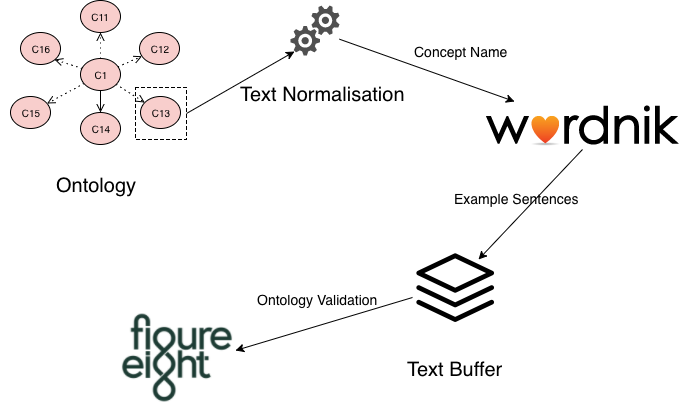
\includegraphics[width=.8\textwidth]{figures/External_Source_Workflow}
							 \caption{Conceptual Model of WordNik consultation to generate Context}
						\end{figure}
						
						\vspace{-1cm}
						\hrulefill
						
						\begin{itemize}
							\small
							\justifying
							\setlength\itemsep{0.5cm}
							\item Context Generation based on {\usebeamercolor[fg]{itemize item}{Dictionary Lookup}}
							\item Fetches Context from the online dictionary {\usebeamercolor[fg]{itemize item}{WordNik}}
							\item Best suited for ontologies containing {\usebeamercolor[fg]{itemize item}{common, well known concepts}}
							\item Often fails when concept names contain phrases or special characters
						\end{itemize}
					\end{minipage}
					\hfill
					\hbox{}
				\end{minipage}
				\vspace{1cm}
			\end{block}
		\end{column}
		
		
		%BOTTOM%
		\begin{columns}[t, onlytextwidth]
			\begin{column}{.49\textwidth}
				\begin{block}{Experimental Evaluation}
					\begin{minipage}[t][.2\textheight][c]{\textwidth}
						
						\hfill
						\begin{minipage}[t]{0.93\textwidth}
							\begin{minipage}[t]{\textwidth}
								\small
								{\usebeamercolor[fg]{itemize item}CS Task Interfaces}
								
								\vspace{-5mm}
								\begin{minipage}[t]{.49\textwidth}
									\begin{figure}[H]
										 \centering
										 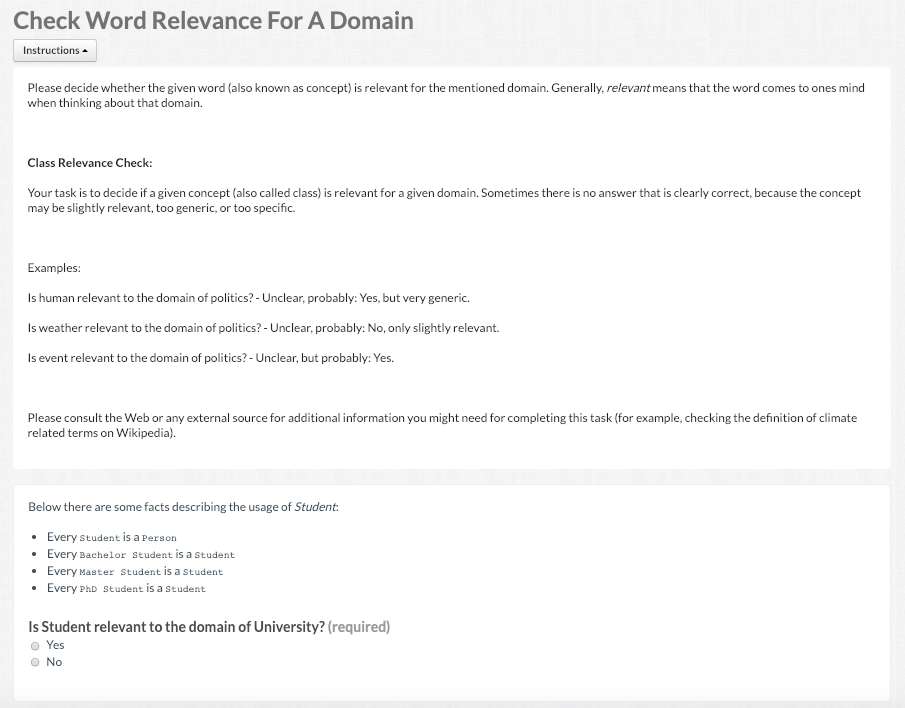
\includegraphics[width=\textwidth]{figures/questionaire_university_example}
										 \caption{Ontology based Approach}
									\end{figure}
								\end{minipage}
								\begin{minipage}[t]{.49\textwidth}
									\begin{minipage}[t]{\textwidth}
										\begin{figure}[H]
											 \centering
											 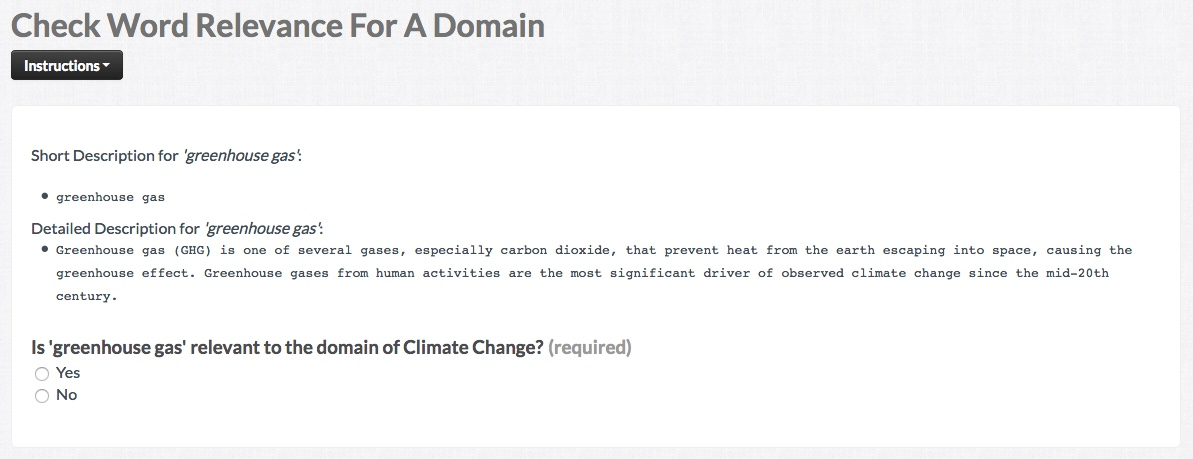
\includegraphics[width=\textwidth]{figures/questionaire_metadata_example}
											 \caption{Metadata based Approach}
										\end{figure}
									\end{minipage}
									\begin{minipage}[t]{\textwidth}
										\vspace{-1.9mm}
										\begin{figure}[H]
										 \centering
										 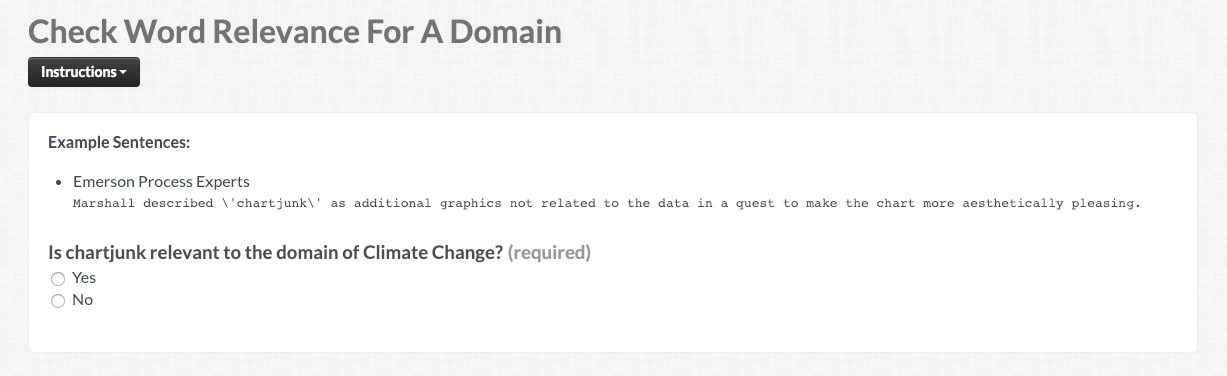
\includegraphics[width=\textwidth]{figures/questionaire_wordnik_example}
										 \caption{Dictionary based Approach}
										\end{figure}
									\end{minipage}
								\end{minipage}
							\end{minipage}
						\end{minipage}
						\hfill
						\hbox{}
						
					\end{minipage}
				\end{block}
			\end{column}
			\begin{column}{.49\textwidth}
				\begin{block}{Test Test}
					\begin{minipage}[t][.2\textheight][c]{\textwidth}
						
					\end{minipage}
				\end{block}
			\end{column}
		\end{columns}
		\begin{columns}[t, onlytextwidth]
			\begin{column}{\textwidth}
				\begin{block}{Conclusion \& Future Work}
					\hfill
					\begin{minipage}[t][.09\textheight][c]{0.97\textwidth}
						\begin{multicols}{2}
							\footnotesize
							{\usebeamercolor[fg]{itemize item}{Improvements through Context Enrichment}}\\
							\vspace{-5mm}
							\begin{itemize}
								\footnotesize
								\justifying
								\setlength\itemsep{5mm}
								\item All 3 approaches improved the performance of the crowd (F-Measure above~80~\%)
								\item The number of misclassified concepts could be reduced in all 3 approaches
								\item The Metadata~based~Approach achieves results of highest quality and facilitates the most flexible Context Generation
							\end{itemize}
							\footnotesize
							{\usebeamercolor[fg]{itemize item}{Future Work}}\\
							\vspace{-1cm}
							\begin{itemize}
								\footnotesize
								\justifying
								\setlength\itemsep{5mm}
								\item (Re-)evaluation of the approaches with realistically large datasets to discover any bias towards specific characteristics of the validated ontology
								\item Development of recommendations and guidelines towards a generic framework which combines the approaches to achieve high quality results
							\end{itemize}
						\end{multicols}
					\end{minipage}
					\hfill
					\hbox{}
				\end{block}
			\end{column}
		\end{columns}
		
			
		
		%REFERENCES
		\begin{columns}[t, onlytextwidth]
			\begin{column}{\textwidth}
				\scriptsize
				
				References:
				
				\vspace{-1cm}
				\setlength{\columnsep}{-10cm}
				\begin{multicols}{2}
					\bibliographystyle{abbrv}
					\bibliography{literature}
				\end{multicols}
			\end{column}
		\end{columns}
		
    \end{column}

  \end{columns}
\end{frame}


\end{document}
